\chapter{Analisys and result discussion}
In the previous section the author has explained the steps followed to forecast electricity prices and explore the different predictors' influence. We are now discussing the configuration fixed for the hourly, daily, monthly and yearly setups, and the results obtained on each case.

For each scenario has to be selected the length of the time series to be used, the forecasting horizon, the number of lags and the predictors to be included. This has been selected with the help of a topic expert, concretely my Thesis' Supervisor.

\section{Hourly analysis}
In this case the author is using data of the previous 6 months. It's been decided to make predictions of 168 hours ahead (1 week). The lags in use try to model the autocorrelation, and are the following: 2, 12, 23, 24, 36, 71, 72, 167 and 168. Apart, other predictors are included to add extra information to the model:

\begin{itemize}
    \item \textbf{Demand:} The total energy demand.
    \item \textbf{Generation:} Wind, hydropower, nuclear, solar, combined cycle and coal generation technologies measurements.
\end{itemize}

Cross validation is applied using 20 windows, with step size of 25.

As the author mentioned, the energy market has changed due to the Covid pandemic and specially to the war in Ukraine. This differences between current and past market will be analyzed.

\subsection{Pre-pandemic scenario}
The data used for the pre-pandemic scenario experiments goes from 2018-10-01 to 2019-03-31, before the increase in energy prices shown in Figure \ref{fig:spot-price-series-month}. In Table \ref{tab:cv-hourly-prep} you can find the performance of different models for the cross validation phase. The best one is a Random Forest, it is the one the author will use to make the final forecast.

\begin{table}[H]
\centering
\begin{tabular}{@{}l|l|l@{}}
\toprule
Model & MASE     & Fit time     \\ \midrule
RF    & 2.76181  & 1940.086432  \\
GBT   & 2.938516 & 14009.034606 \\
kNN   & 3.939263 & 17.24593     \\
SVR   & 4.252531 & 5547.920132  \\
DR    & 4.741289 & 4.483376     \\ \bottomrule
\end{tabular}
\caption{Model performance comparison trained over the hourly pre-pandemic energy price.}
\label{tab:cv-hourly-prep}
\end{table}

The final forecast is done as explained in Chapter \ref{ch:methodology}, using the train split to build the model and the test to give a final evaluation of the performance. The results are shown in Figure \ref{fig:forecast-hourly-pre}, obtaining a MASE=2.23.

\begin{figure}[H]
\centering
    \caption{Final forecasting of hourly pre-pandemic energy price.}
    \label{fig:forecast-hourly-pre}
    \fbox{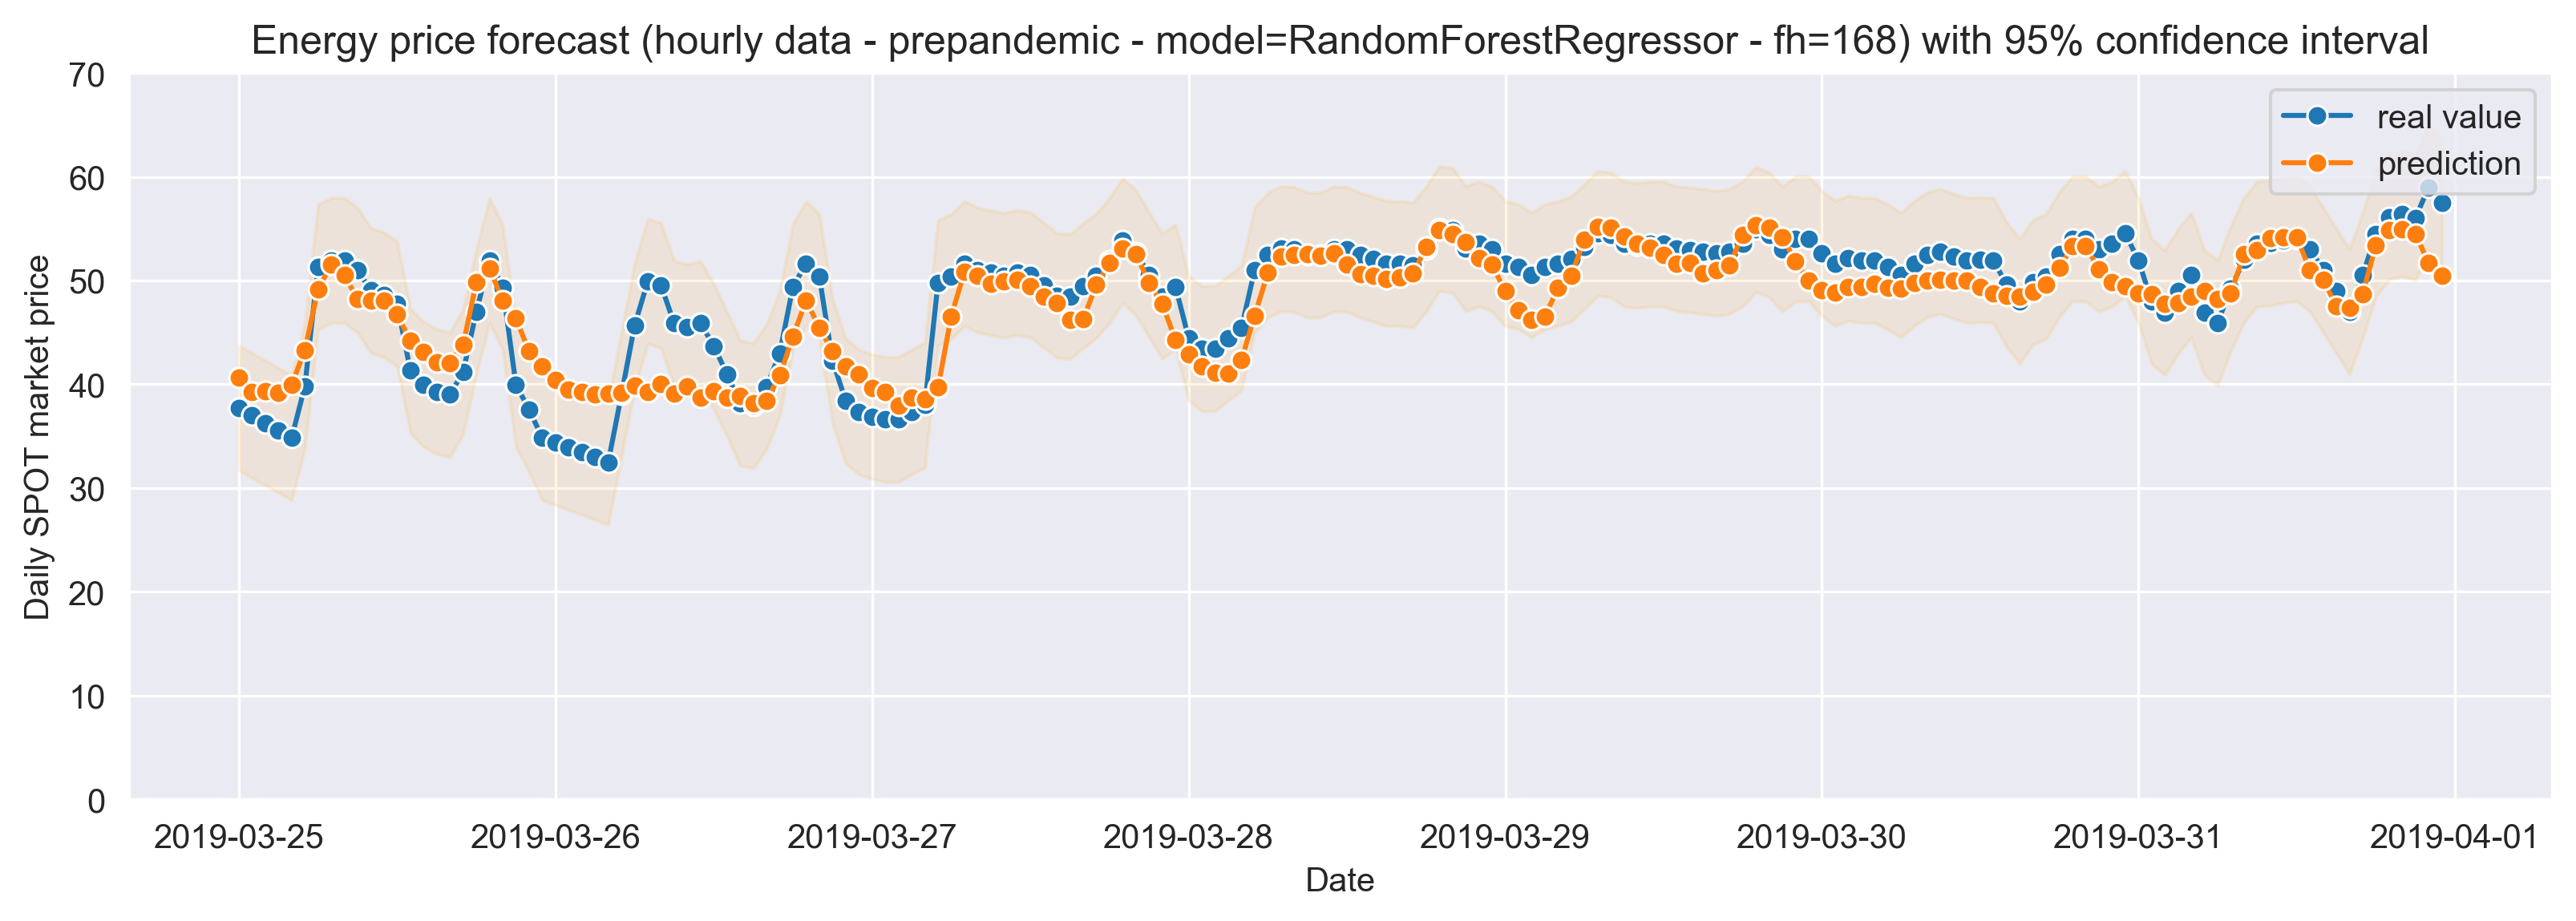
\includegraphics[scale=0.4]{images/analysis/forecast-hourly-pre}}
\end{figure}

Which are the predictors that are specially influencing this forecast? In Figure \ref{fig:shap-hourly-pre} you can see them, both for fh=1 and fh=168.

In the first case, the first lag has a lot of importance, high SHAP values are found for many test points. Concretely, if the lag takes a low value (blue color), the response value will tend to be low too. Lag two has also some importance, but in this case a low value in the lag means a higher value in the response. Combined cycle generation and hour seem to have some importance, but not very high.

In the second case, the forecast is not so dependent of the first lag, as the response (fh=168) is further away from it. Combined cycle, coal and hydropower generation are the most influential in the price.

\begin{figure}[H]
\centering
    \begin{subfigure}{.45\textwidth}
        \centering
        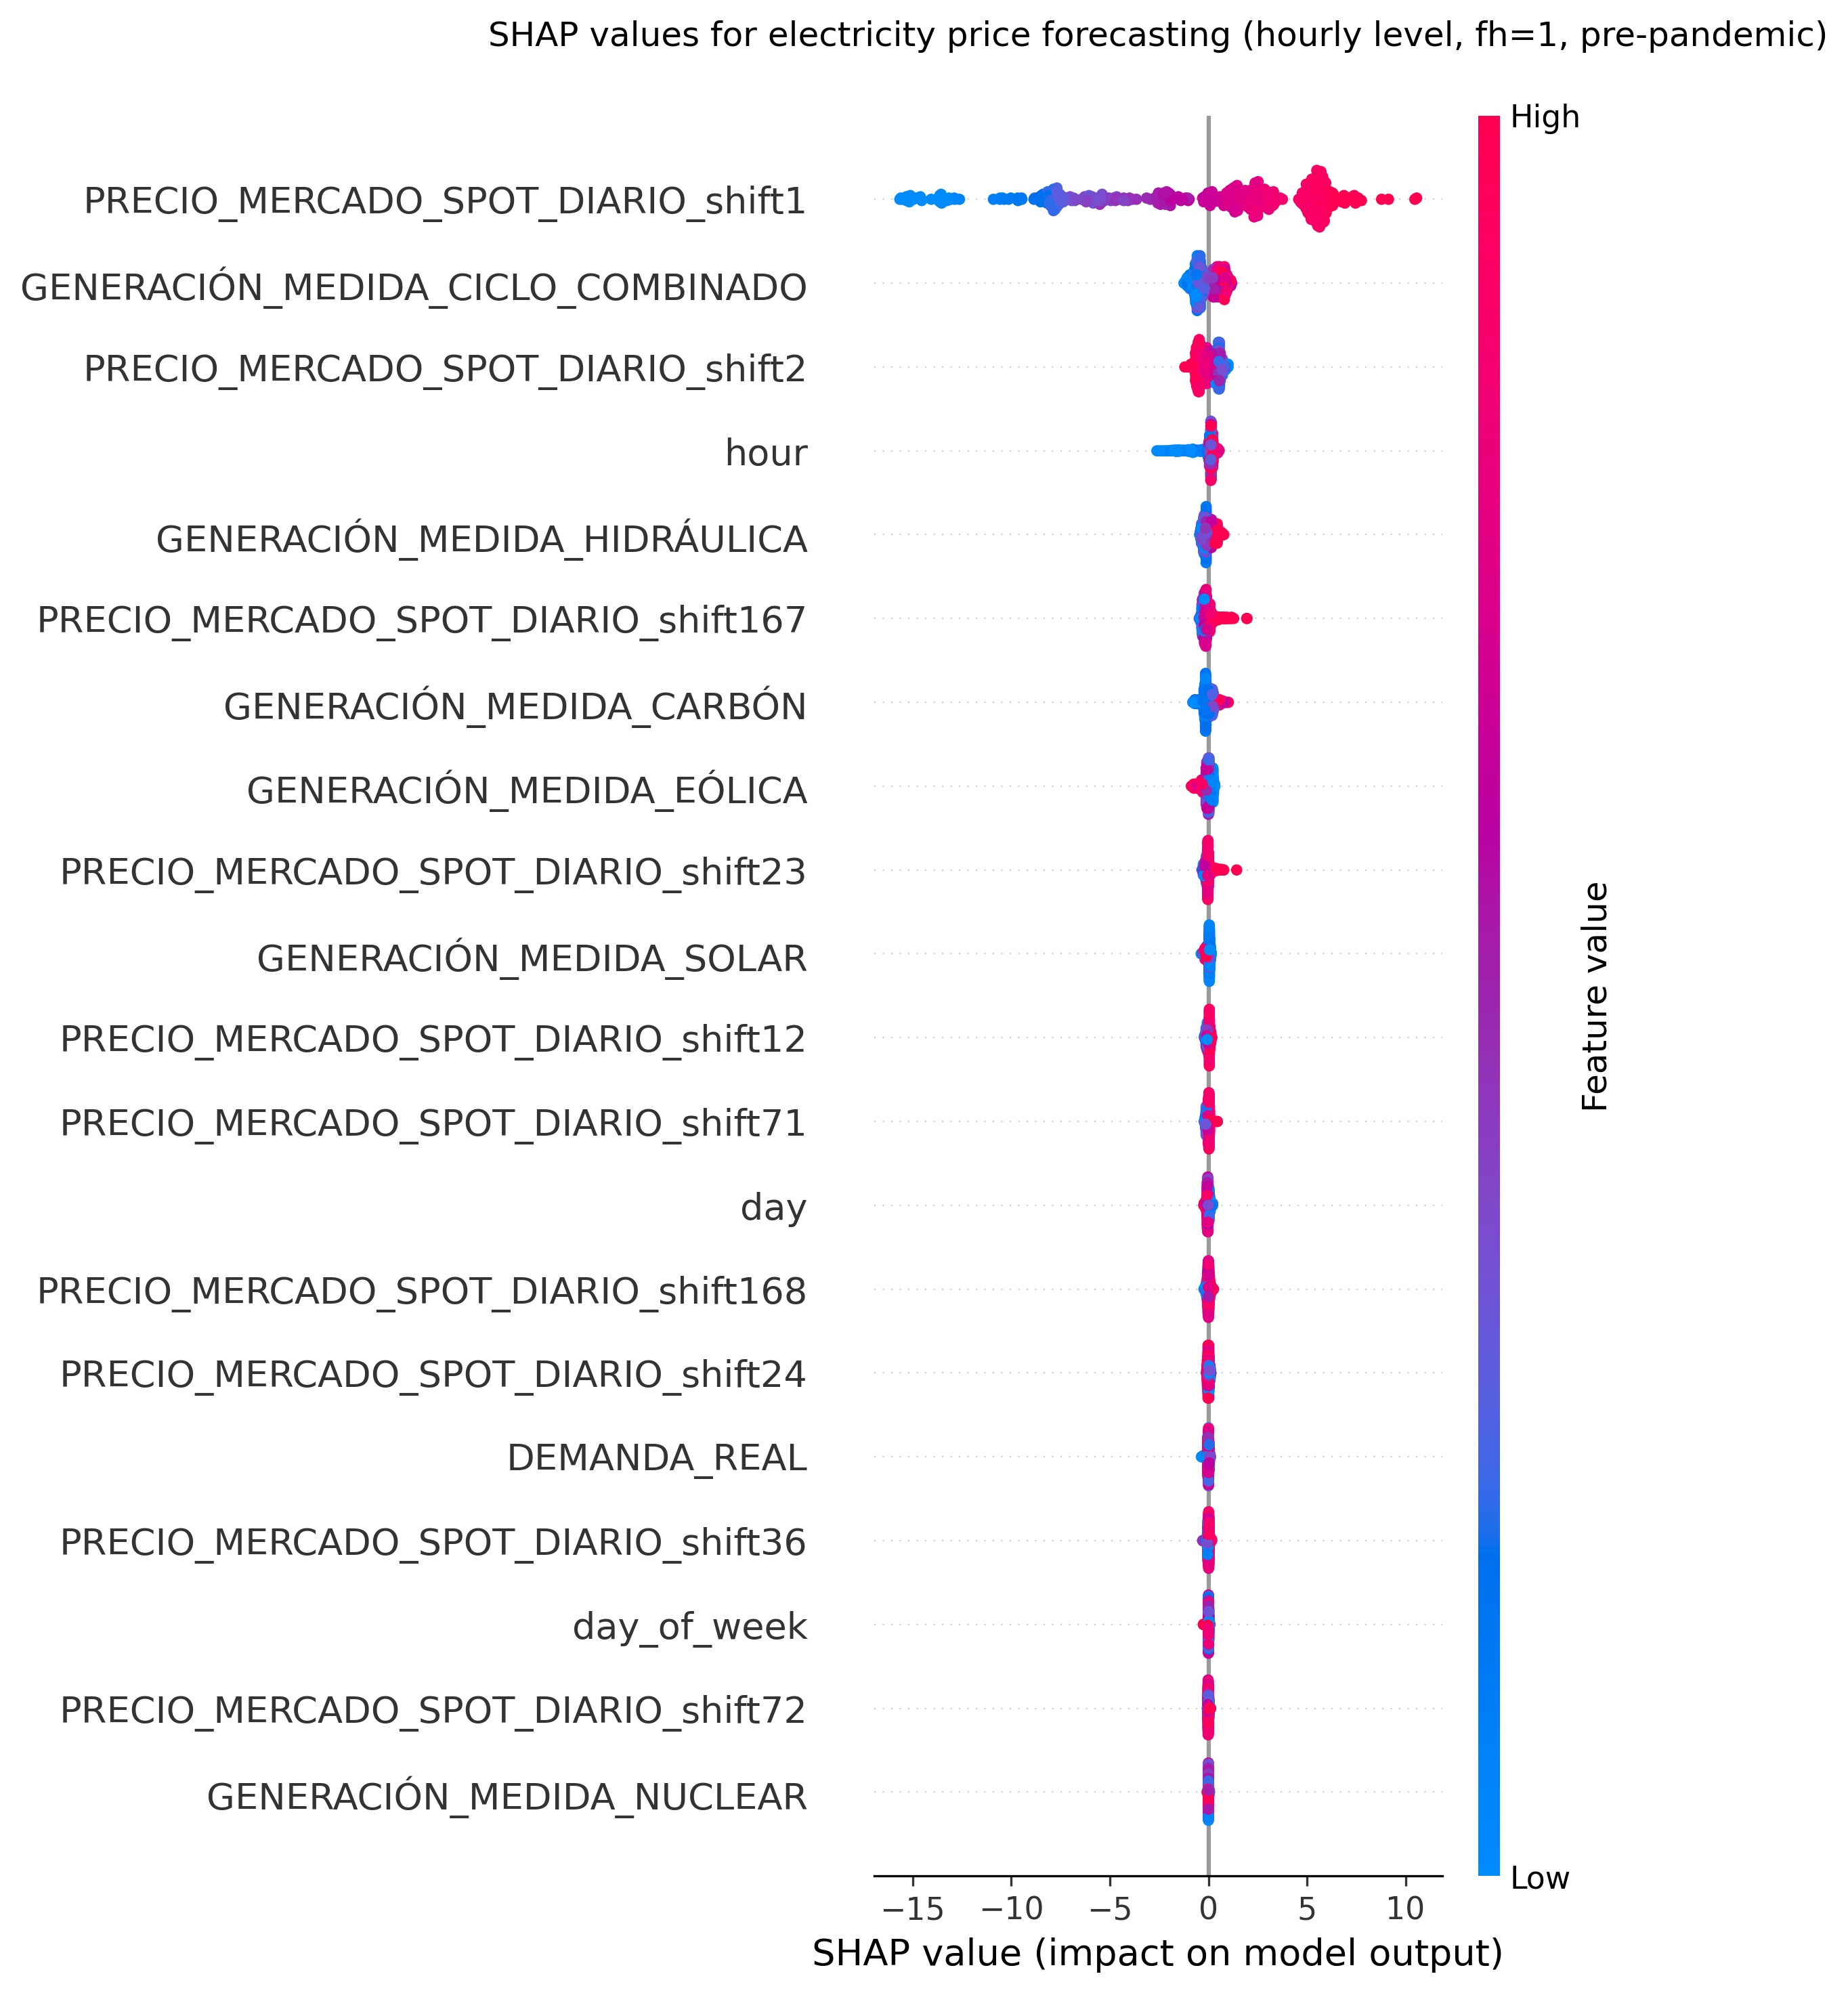
\includegraphics[width=1\linewidth]{images/analysis/shap-hourly-pre-1}
        \caption{fh=1}
    \end{subfigure}
    \begin{subfigure}{.45\textwidth}
        \centering
        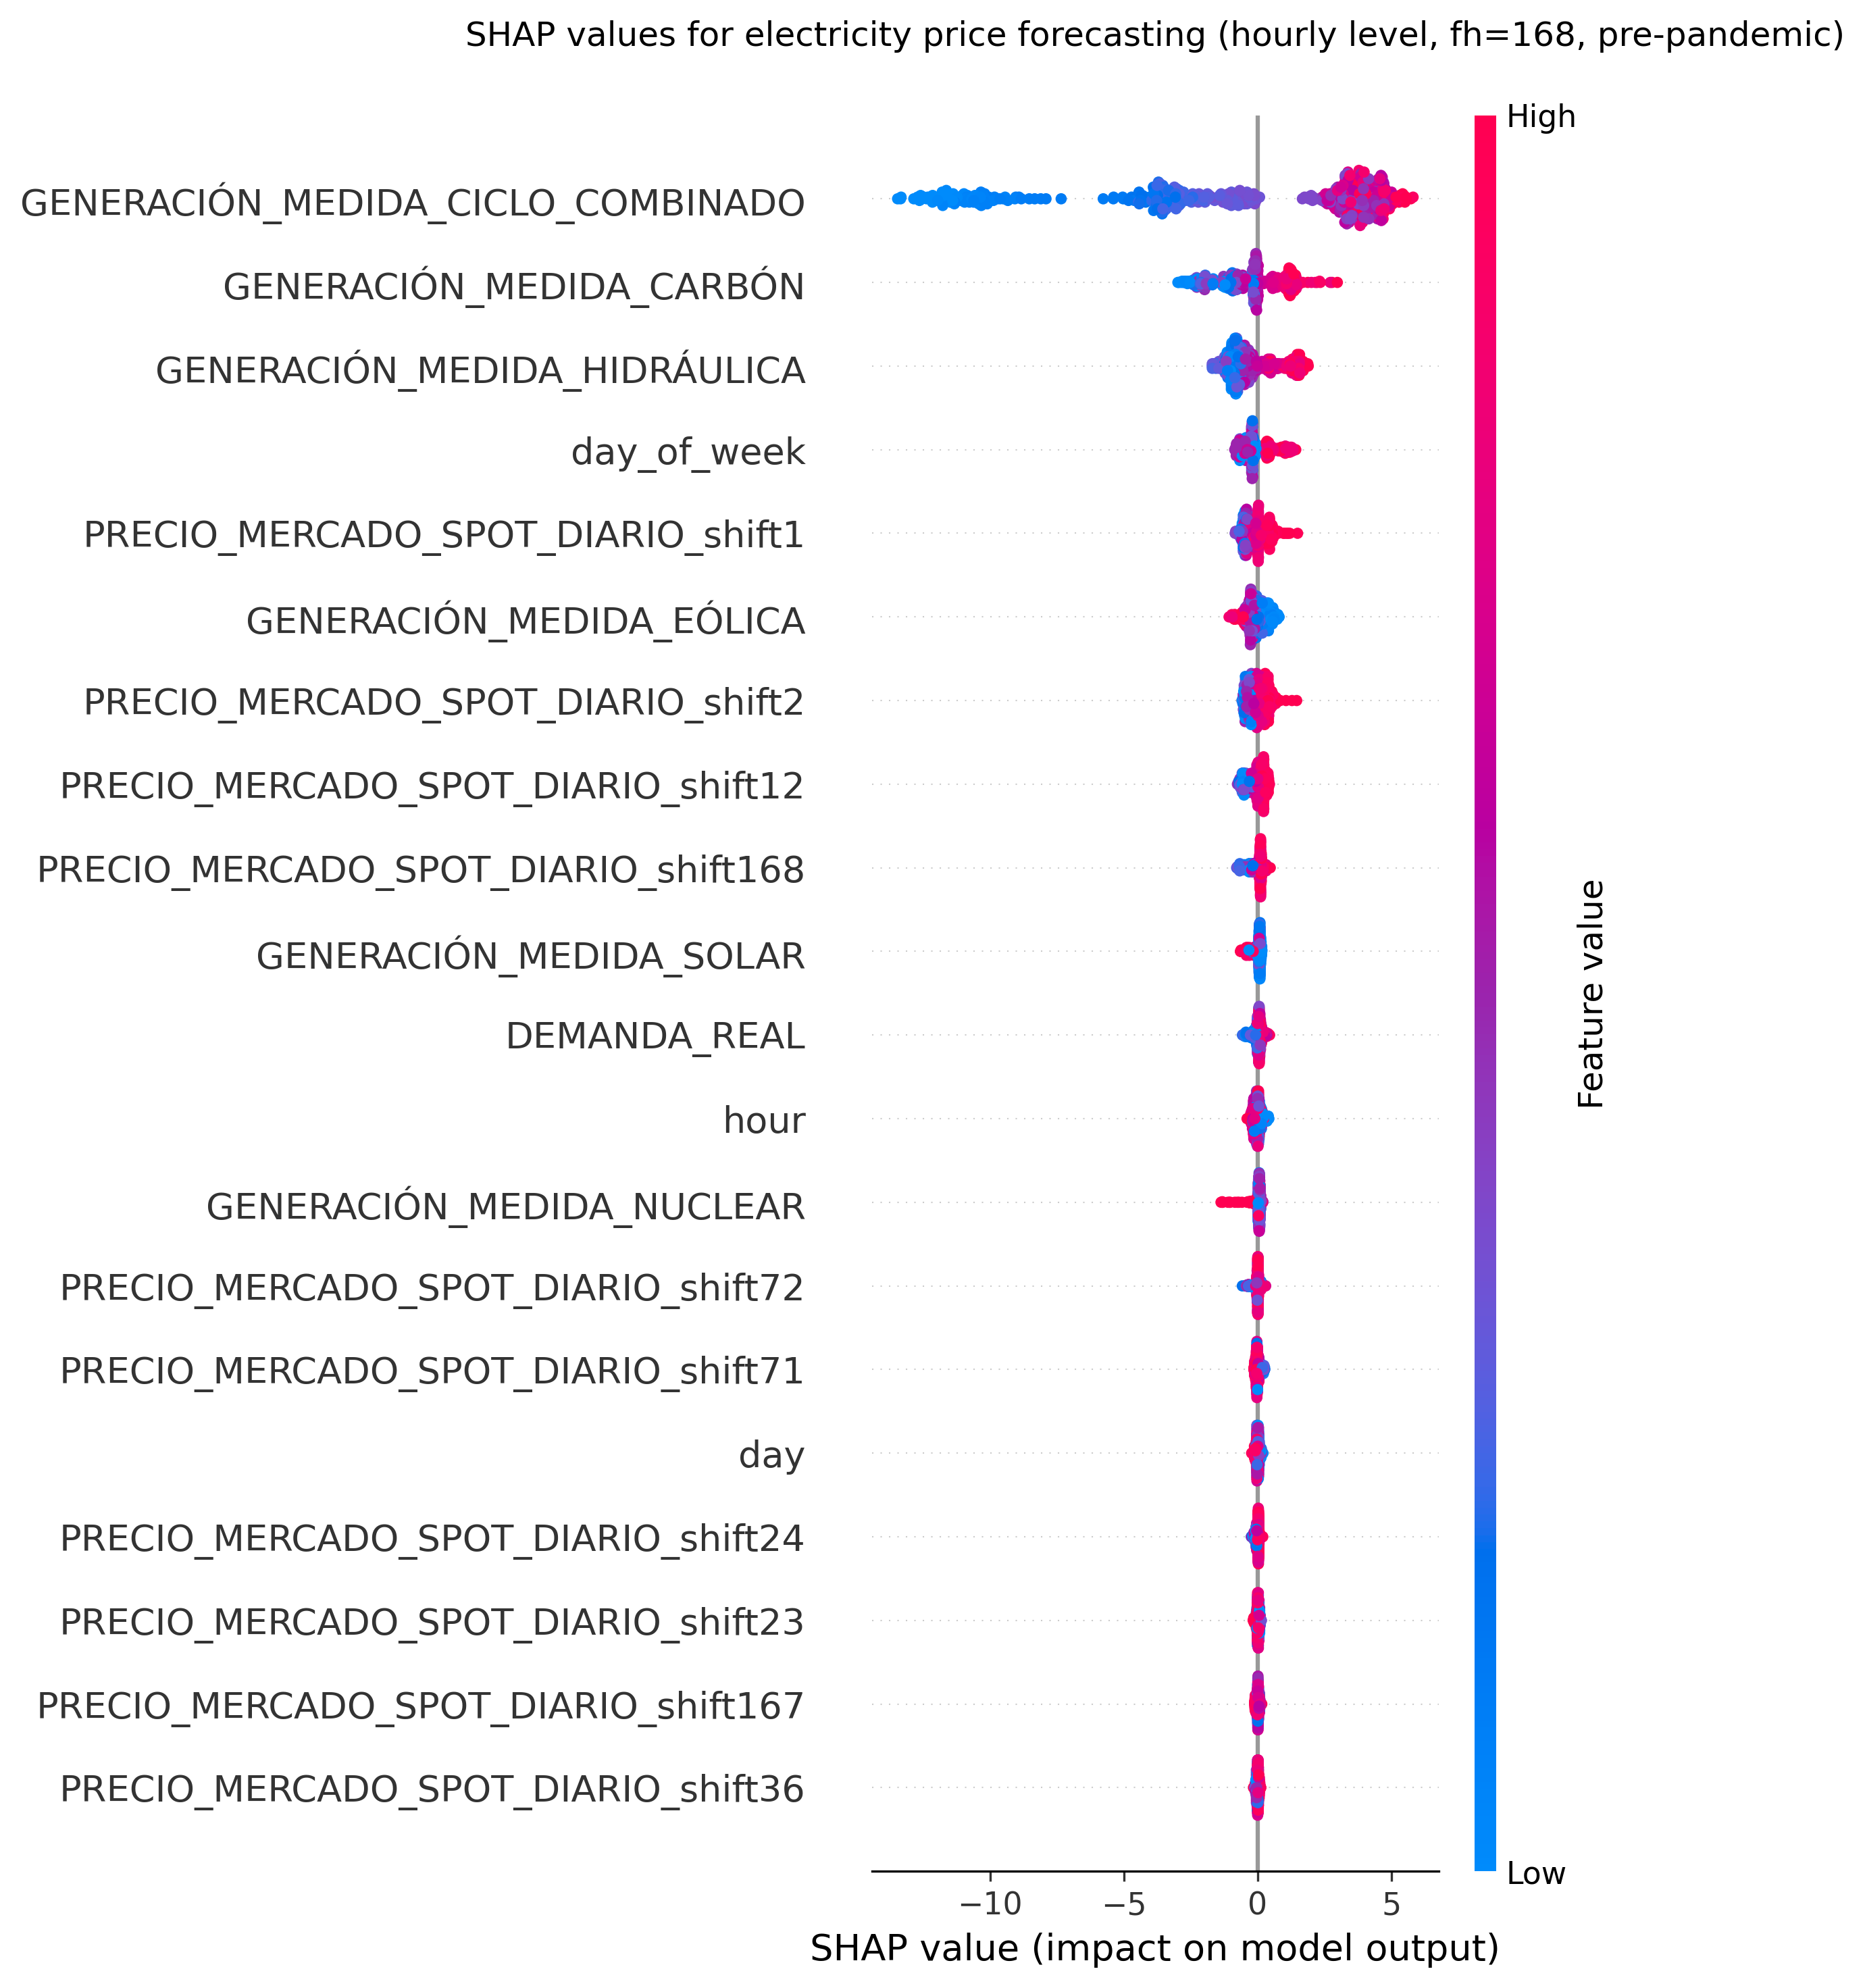
\includegraphics[width=1\linewidth]{images/analysis/shap-hourly-pre-168}
        \caption{fh=168}
    \end{subfigure}

    \caption{SHAP values for the hourly pre-pandemic energy price forecasting.}
    \label{fig:shap-hourly-pre}
\end{figure}

\subsection{Post-Unkraine war scenario}
The data in use goes from 2022-10-01 to 2023-03-31. In the model selection stage the author obtains the results described in Table \ref{tab:cv-hourly-post}.

% Please add the following required packages to your document preamble:
% \usepackage{booktabs}
\begin{table}[H]
\centering
\begin{tabular}{@{}l|l|l@{}}
\toprule
Model & MASE     & Fit time     \\ \midrule
GBT   & 3.713739 & 5196.343993  \\
RF    & 3.755286 & 13717.128606 \\
SVM   & 3.901001 & 2823.434254  \\
kNN   & 3.932622 & 3.564837     \\
DR    & 4.770888 & 7.018414     \\ \bottomrule
\end{tabular}
\caption{Model performance comparison trained over the hourly post-Ukraine war energy prices.}
\label{tab:cv-hourly-post}
\end{table}

The best-performing model, in this post-war scenario, is the one based on Gradient Boosted Trees (GBT). The final forecast is shown in Figure \ref{fig:forecast-hourly-post} with a MASE of 4.01.

\begin{figure}[H]
\centering
    \caption{Final forecasting of hourly post-war energy price.}
    \label{fig:forecast-hourly-post}
    \fbox{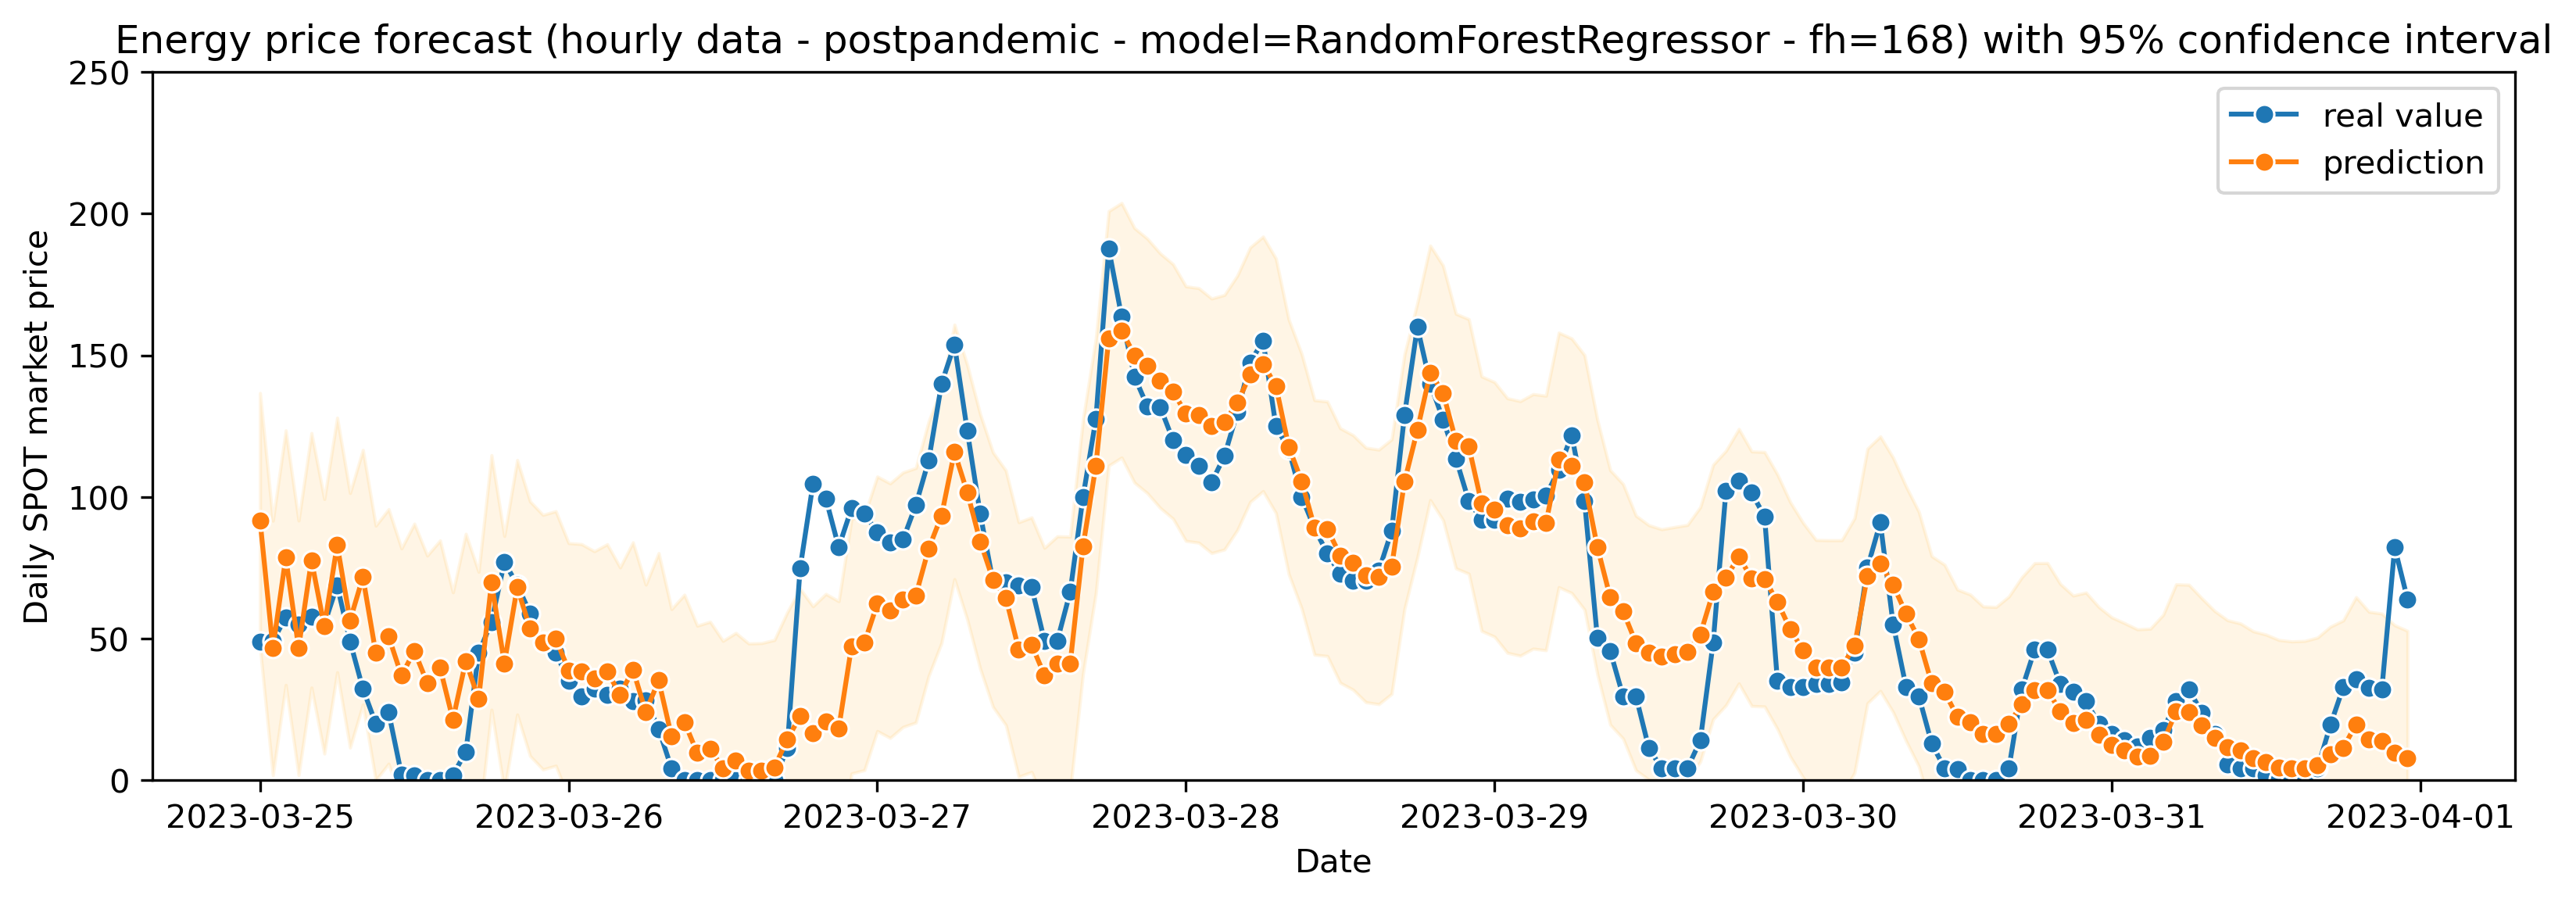
\includegraphics[scale=0.4]{images/analysis/forecast-hourly-post}}
\end{figure}

In this case, the most important predictors are shown in Figure \ref{fig:shap-hourly-post}. Compared to the pre-pandemic series, we find similar predictors for fh=1, but with higher weight for combined cycle generation. For fh=168, combined cycle generation is also increasing its repercussion in prices. This makes sense, as gas prices have increased a lot and the electricity price series have done it too.

\begin{figure}[H]
\centering
    \begin{subfigure}{.45\textwidth}
        \centering
        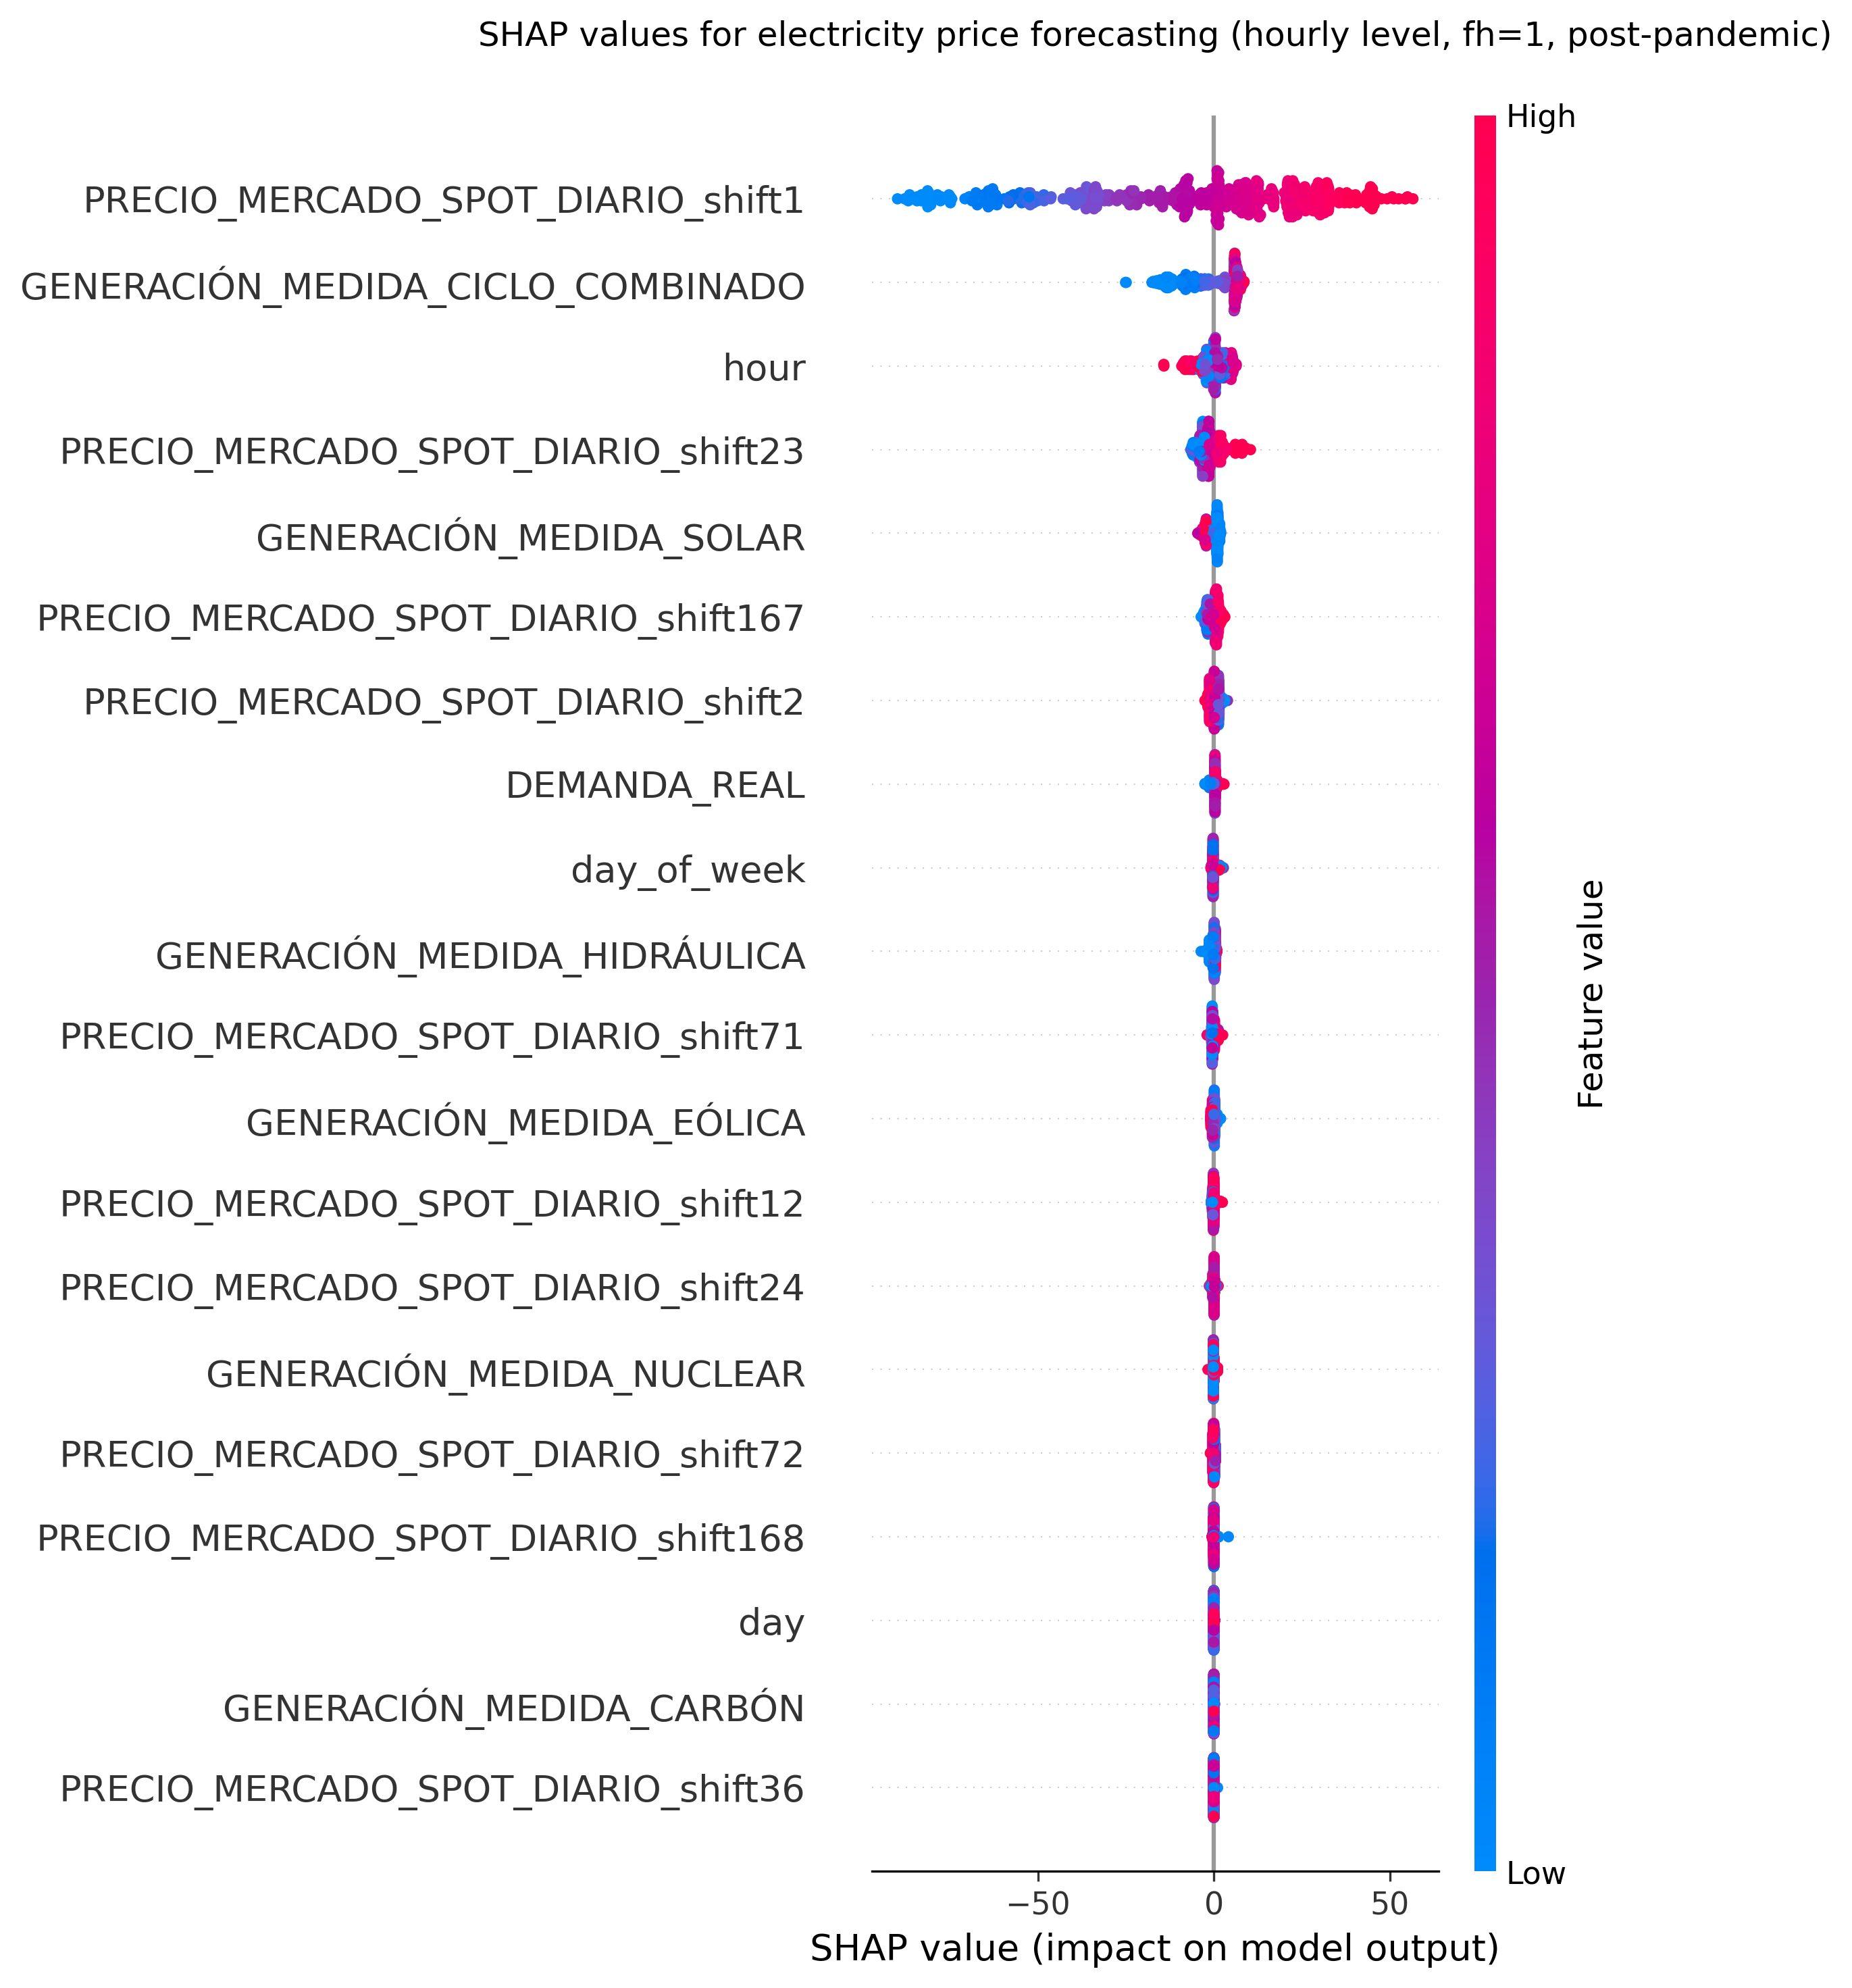
\includegraphics[width=1\linewidth]{images/analysis/shap-hourly-post-1}
        \caption{fh=1}
    \end{subfigure}
    \begin{subfigure}{.45\textwidth}
        \centering
        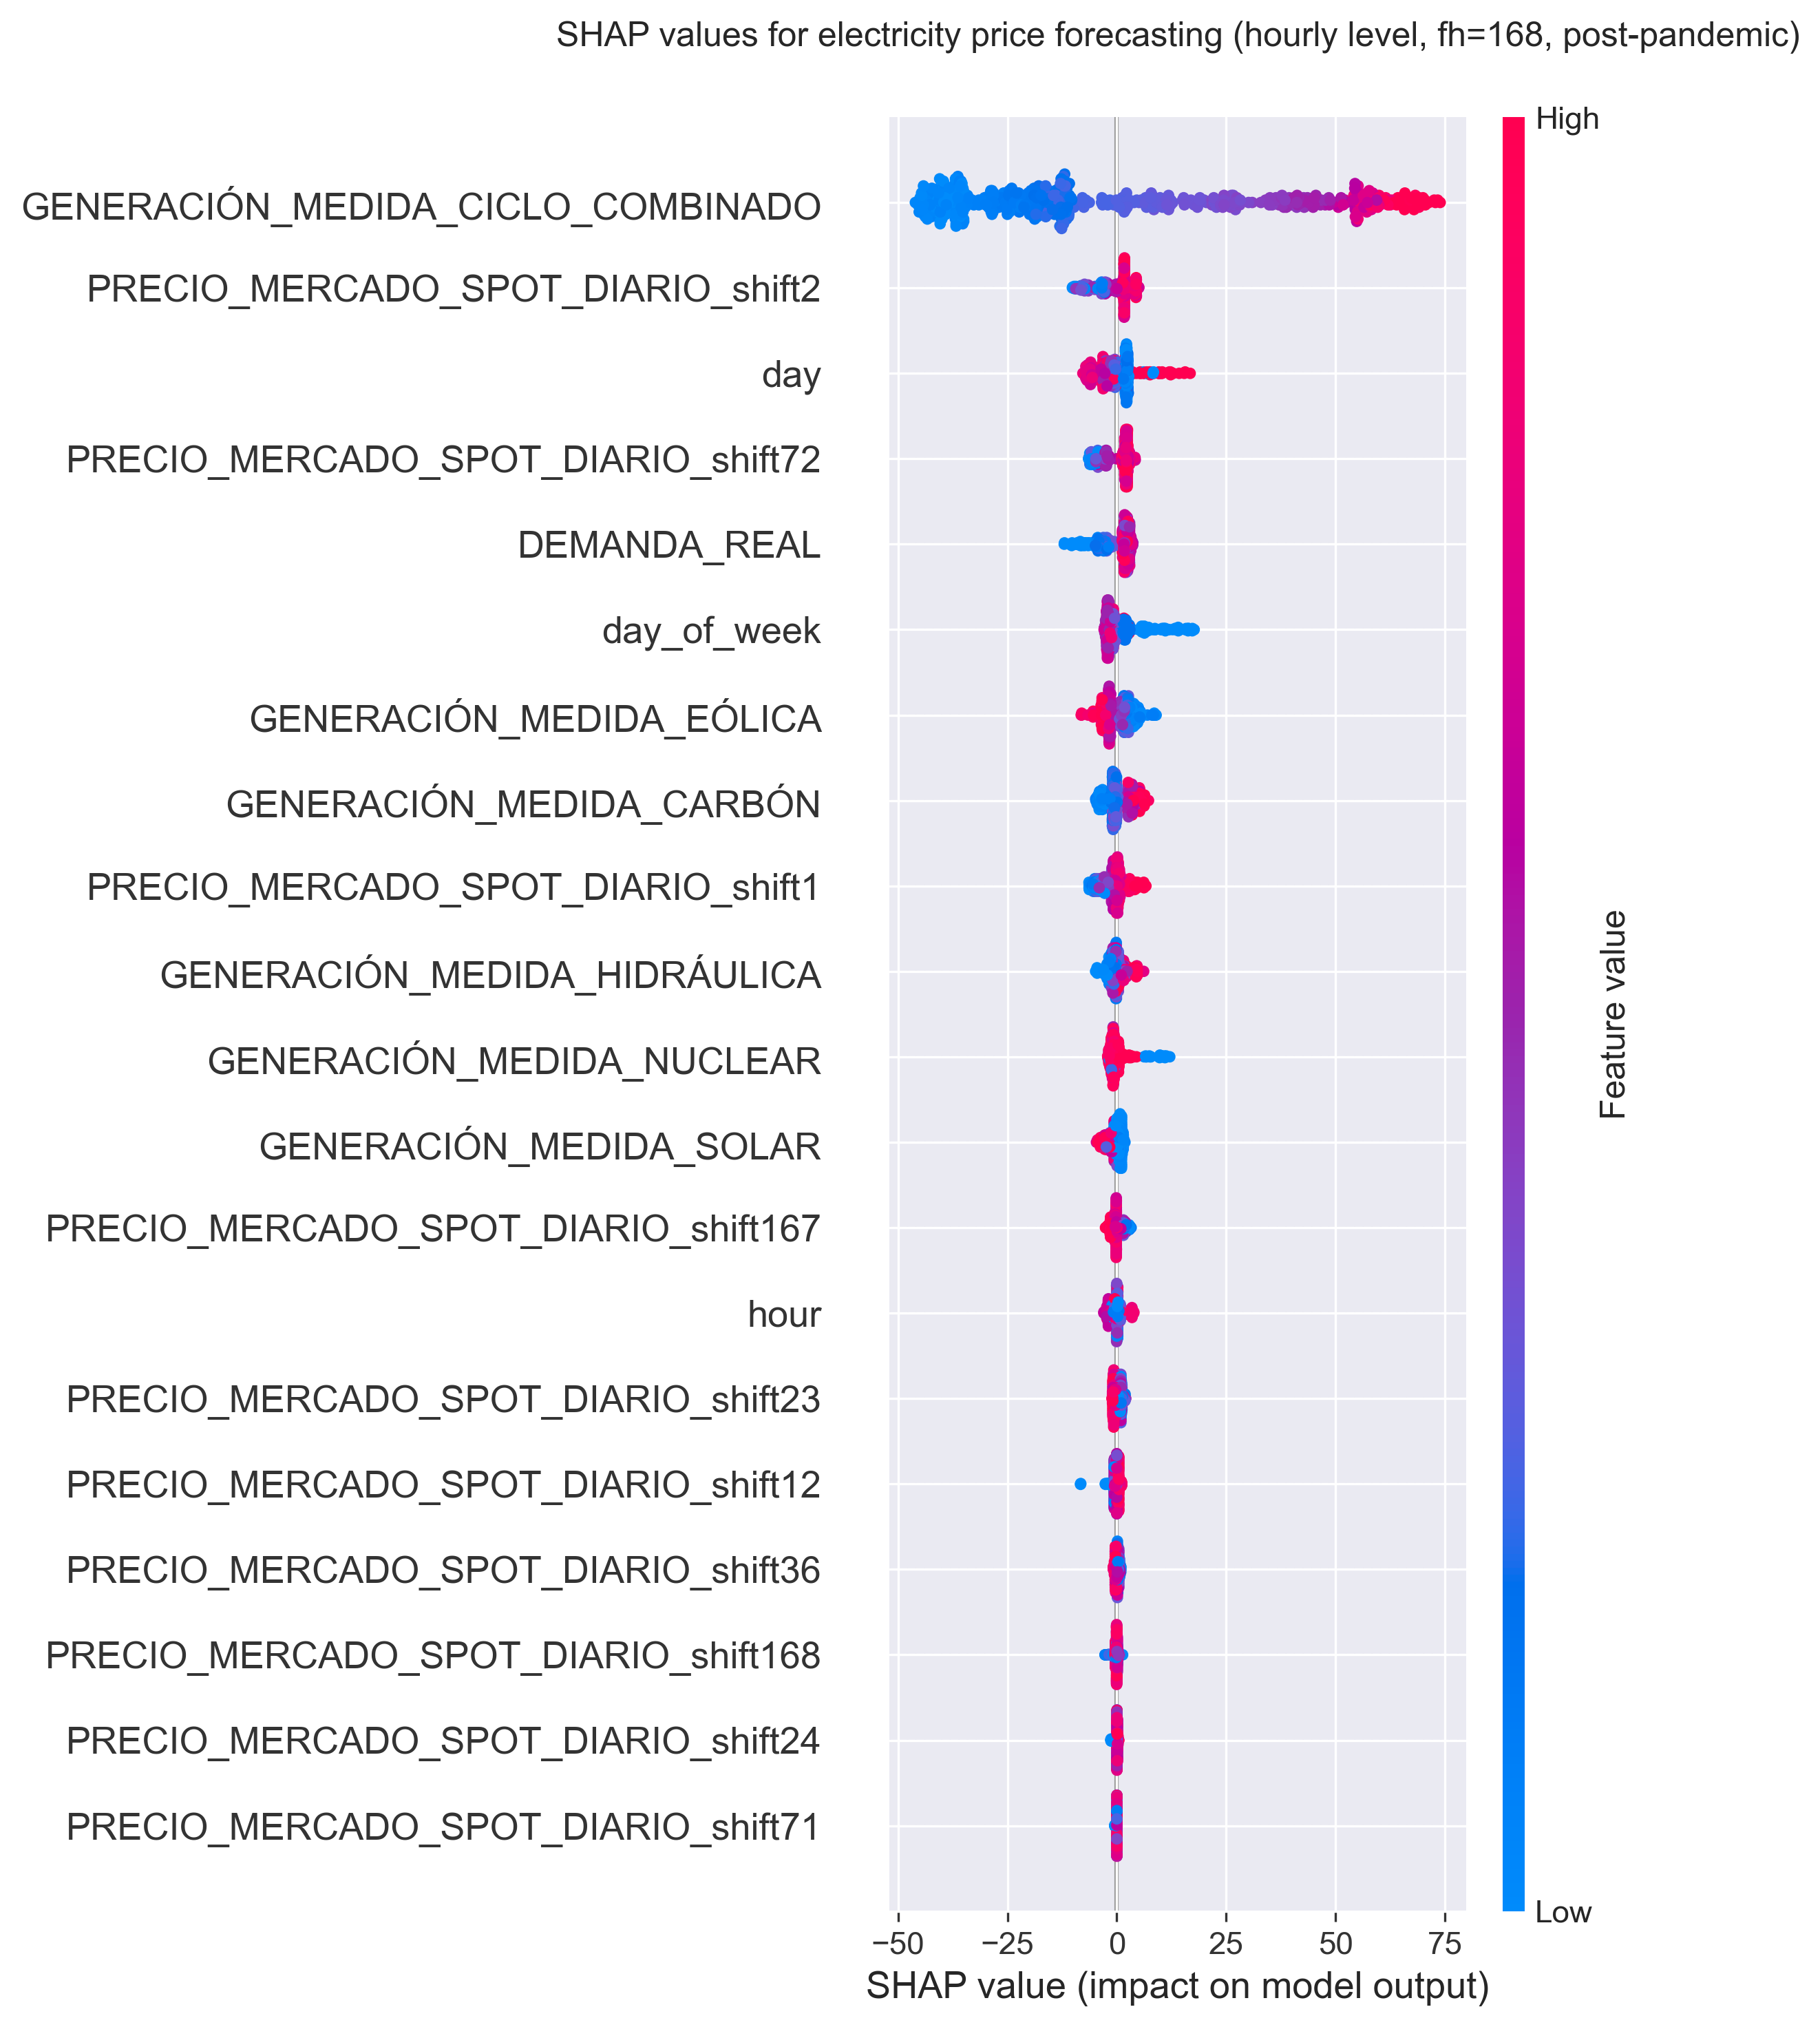
\includegraphics[width=1\linewidth]{images/analysis/shap-hourly-post-168}
        \caption{fh=168}
    \end{subfigure}

    \caption{SHAP values for the hourly post-pandemic energy price forecasting.}
    \label{fig:shap-hourly-post}
\end{figure}


\subsection{Result discussion}
The models that have performed the best are those related with tree ensembles, both RF and GBT. With them, reasonably good forecasts have been obtained, getting a low MASE score. Finally, the main difference in the influence of predictors before and after Covid crisis and the war in Ukraine is that now the gas price is affecting more the electricity price than before.


\section{Daily analysis}

\subsection{Pre-pandemic scenario}

\subsection{After-Unkraine war scenario}

\subsection{Result discussion}


\section{Monthly analysis}


\section{Yearly analysis}